\newif\ifvimbug
\vimbugfalse

\ifvimbug
\begin{document}
\fi


\subsection{Interpolation in verschiedenen Darstellungsformen (5 Punkte)}
\subsubsection{1 Punkt}
$Va = P$\\
\\
$\begin{pmatrix}
1 & 0 & 0 \\ 
1 & 2 & 4 \\ 
1 & 4 & 16
\end{pmatrix} \begin{pmatrix}
a_{0} \\ 
a_{1} \\ 
a_{2}
\end{pmatrix} = \begin{pmatrix}
1&0 \\ 
3&2 \\ 
2&4
\end{pmatrix} $\\
\\
$a =V^{-1} P$:\\
\\
$ \begin{pmatrix}
a_{0} \\ 
a_{1} \\ 
a_{2}
\end{pmatrix} = \begin{pmatrix}
1 &0 & 0 \\ 
\frac{-3}{4} & 1 & \frac{-1}{4} \\ 
\frac{1}{8} & \frac{-1}{4} & \frac{1}{8}
\end{pmatrix} *\begin{pmatrix}
1&0 \\ 
3&2 \\ 
2&4
\end{pmatrix} $\\
Daraus folgt Polynom:\\
$$P_{M}(t) = - \begin{pmatrix}\frac{3}{8}\\0\end{pmatrix}t^{2} + \begin{pmatrix}\frac{7}{4}\\1\end{pmatrix}t + \begin{pmatrix}1\\0\end{pmatrix}$$

Auswertung weiterer Punkte:
$$P_{M}(1) = -\begin{pmatrix}\frac{3}{8}\\0\end{pmatrix} + \begin{pmatrix}\frac{7}{4}\\1\end{pmatrix} + \begin{pmatrix}1\\0\end{pmatrix} = \begin{pmatrix}\frac{19}{8}\\1\end{pmatrix}  $$
$$P_{M}(3) = -\begin{pmatrix}\frac{3}{8}\\0\end{pmatrix}9 + \begin{pmatrix}\frac{7}{4}\\1\end{pmatrix}3 + \begin{pmatrix}1\\0\end{pmatrix} =  \begin{pmatrix}\frac{23}{8}\\3\end{pmatrix}$$ 
$$P_{M}(5) = -\begin{pmatrix}\frac{3}{8}\\0\end{pmatrix}25 + \begin{pmatrix}\frac{7}{4}\\1\end{pmatrix}5 + \begin{pmatrix}1\\0\end{pmatrix} =  \begin{pmatrix}\frac{3}{8}\\5\end{pmatrix}$$ 

In Rot die Orginalen Stützstellen. in Blau die neu berechneten.\\
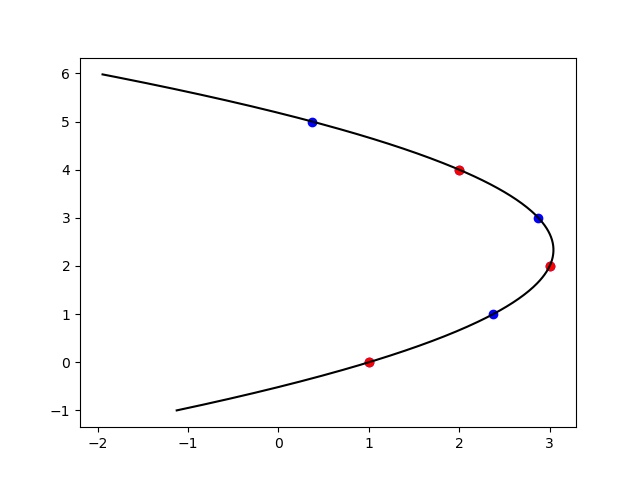
\includegraphics[width=\linewidth]{1a}
\subsubsection{1 Punkt}
$$l_{i}(t) = {\displaystyle \prod_{j=0,j \neq i}^{q}} \dfrac{t - t_{j}}{t_{i} - t_{j}}$$
$$l_{0}(t) = \dfrac{t - 2}{0 - 2} * \dfrac{t - 4}{0 - 4} = \dfrac{t^{2} - 6*t + 8}{8}$$
$$l_{1}(t) = \dfrac{t - 0}{2 - 0} * \dfrac{t - 4}{2 - 4} = \dfrac{t^{2} - 4*t }{-4}$$
$$l_{2}(t) = \dfrac{t - 0}{4 - 0} * \dfrac{t - 2}{4 - 2} = \dfrac{t^{2} - 2*t }{8}$$
$$P_{L}(t) = {\displaystyle \sum_{i=0}^{q}} l_{i}(t)P_{i} $$
$$P_{L}(t) = \dfrac{t^{2} - 6*t + 8}{8}*\begin{pmatrix}1\\0\end{pmatrix} + \dfrac{t^{2} - 4*t }{-4}*\begin{pmatrix}3\\2\end{pmatrix}  +  \dfrac{t^{2} - 2*t }{8} *\begin{pmatrix}2\\4\end{pmatrix} $$
$$ = \begin{pmatrix}
\dfrac{t^{2} - 6*t + 8}{8} + 3*\dfrac{t^{2} - 4*t }{-4} + 2*\dfrac{t^{2} - 2*t }{8}\\
2*\dfrac{t^{2} - 4*t }{-4} + 4*\dfrac{t^{2} - 2*t }{8}
\end{pmatrix} $$
$$ = \begin{pmatrix}
\dfrac{t^{2} - 6*t + 8 - 6t^2 +24t + 2t^2 -4t^2}{8}\\
\dfrac{-4t^{2} + 16*t  + 4t^{2} - 8*t }{8}
\end{pmatrix} $$
$$ = \begin{pmatrix}
\dfrac{-3t^2 +14t + 8}{8}\\
t
\end{pmatrix} $$
$$ = \begin{pmatrix}
\dfrac{-3}{8}t^2 +\dfrac{7}{4}t + 1\\
t
\end{pmatrix} $$
Offensichtlich sind $P_{M}(t)$ und $P_{L}(t)$ identisch.
\subsubsection{1 Punkt}
\begin{tikzpicture}[grow=left,
level 1/.style={sibling distance=15mm},edge from parent/.style={-,draw},>=latex, level 3/.style={edge from child/.style={->,draw},sibling distance=15mm}]

\node[root] {$\begin{pmatrix}-\frac{3}{8}\\0\end{pmatrix}$}
     child {node[level 2] (c1) {$\begin{pmatrix}+1\\+1\end{pmatrix}$}
           child {node[level 2] (c11) {$\begin{pmatrix}1\\0\end{pmatrix}$}
                 child {node[level 3] (c111) {$0$}}
             }
       child {node[level 2] (c21) {$\begin{pmatrix}3\\2\end{pmatrix}$}
      		child {node[level 3] (c112) {$2$}
      			child {node[level 3] (c1111) {$2$}
      				child {node[level 3] (c11111) {$4$}}
      			}
      			child {node[level 3] (c222) {$2$}}
      		}
             }
       }
 child {node[level 2] (c2) {$\begin{pmatrix}-\frac{1}{2}\\+1\end{pmatrix}$}
       child {node[level 2] (c21) {$\begin{pmatrix}3\\2\end{pmatrix}$}}
       child {node[level 2] (c22) {$\begin{pmatrix}2\\4\end{pmatrix}$}
             child {node[level 3] (c221) {$4$}}
             }
       };
       \draw[-, draw] (c1111) -- (c111);
       \draw[-, draw] (c222) -- (c221);
       \draw[-, draw] (c11111) -- (c222);
\end{tikzpicture}\\
$$P_{N}(t) = \begin{pmatrix}1\\0\end{pmatrix} +\begin{pmatrix}1\\1\end{pmatrix}*t + \begin{pmatrix}-\frac{3}{8}\\0\end{pmatrix}*t(t-2)$$
$$ = \begin{pmatrix}
\dfrac{-3}{8}t^2 +\dfrac{7}{4}t + 1\\
t
\end{pmatrix} $$
Das Polynom $P_{N}(t)$ ist identisch $P_{M}(t)$ und $P_{L}(t)$.
\subsubsection{2 Punkte}
Die Newton-Darstellung lässt sich am einfachsten erweitern, da man dem Dreiecksschema ohne viel Aufwand eine neue Stützstelle hinzufügen kann. \\
\begin{tikzpicture}[grow=left,
level 1/.style={sibling distance=15mm},edge from parent/.style={-,draw},>=latex, level 3/.style={edge from child/.style={->,draw},sibling distance=15mm}]

\node[root] {$\begin{pmatrix}\frac{23}{24}\\0\end{pmatrix}$}
     child {node[level 2] (c1) {$\begin{pmatrix}-\frac{3}{8}\\0\end{pmatrix}$}
           child {node[level 2] (c11) {$\begin{pmatrix}+1\\+1\end{pmatrix}$}
           	child {node[level 2] (c111) {$\begin{pmatrix}1\\0\end{pmatrix}$}}
           	child {node[level 2] (c211) {$\begin{pmatrix}3\\2\end{pmatrix}$}}
             }
       child {node[level 2] (c21) {$\begin{pmatrix}-\frac{1}{2}\\1\end{pmatrix}$}
       		child {node[level 2] (c211) {$\begin{pmatrix}3\\2\end{pmatrix}$}}
       		child {node[level 2] (c311) {$\begin{pmatrix}2\\4\end{pmatrix}$}}
             }
       }
 child {node[level 2] (c2) {$\begin{pmatrix}+\frac{15}{2}\\0\end{pmatrix}$}
       child {node[level 2] (c21) {$\begin{pmatrix}-\frac{1}{2}\\1\end{pmatrix}$}
       		}
       child {node[level 2] (c22) {$\begin{pmatrix}+2\\+1\end{pmatrix}$}
              		child {node[level 2] (c311) {$\begin{pmatrix}2\\4\end{pmatrix}$}}
              		child {node[level 2] (c411) {$\begin{pmatrix}0\\3\end{pmatrix}$}}
             }
       };

\end{tikzpicture}\\

$$P_{N_2}(t) = P_{N}(t) + \begin{pmatrix}-\frac{3}{8}\\0\end{pmatrix} * w_3(t)$$
$$= \begin{pmatrix}\dfrac{-3}{8}t^2 +\dfrac{7}{4}t + 1\\t\end{pmatrix} + \begin{pmatrix}\frac{23}{24}\\0\end{pmatrix} * t(t-2)(t-4)$$
$$= \begin{pmatrix}\dfrac{-3}{8}t^2 +\dfrac{7}{4}t + 1\\t\end{pmatrix} + \begin{pmatrix}\frac{23}{24} * t^3 - \frac{23}{4} * t^2 + \frac{23}{3} * t\\0\end{pmatrix} $$
$$= \begin{pmatrix}\frac{23}{24} * t^3 - \frac{49}{8} * t^2 + \frac{113}{12} * t + 1\\t\end{pmatrix}$$
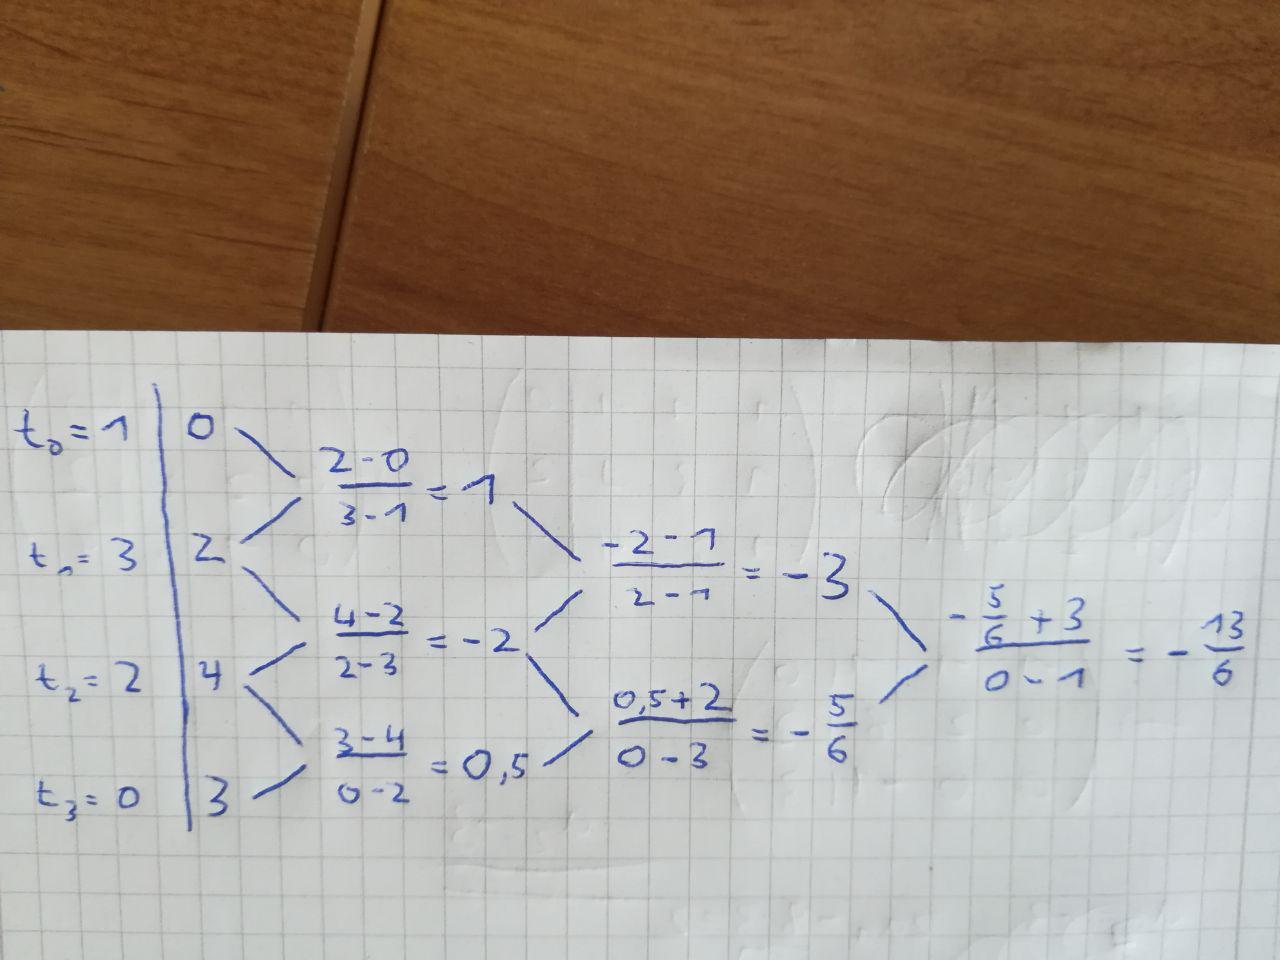
\includegraphics[width=\linewidth]{1d}